% Native TikZ Vector Diagram: 3-Round Non-Overlapping Walk-Forward Timeline (2013-2020)
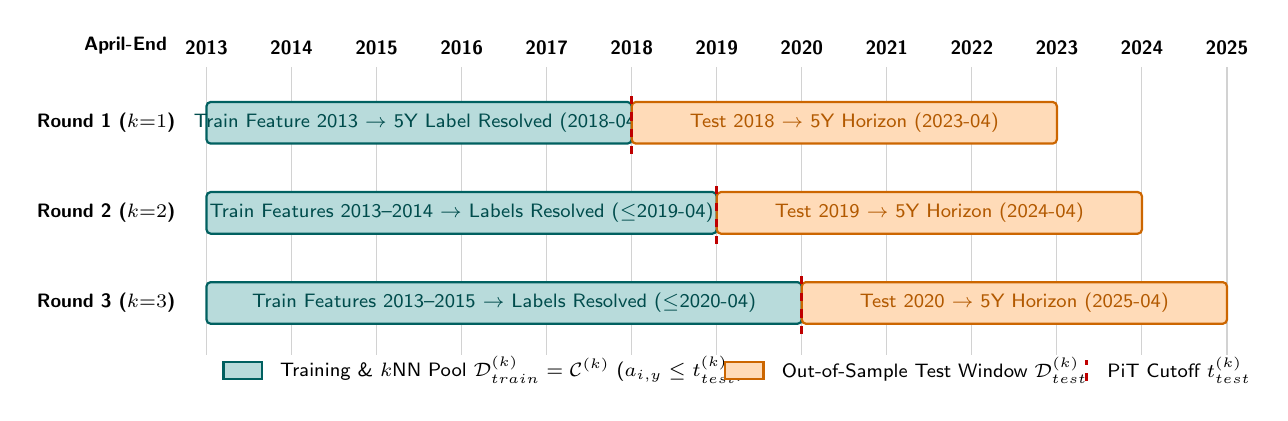
\begin{tikzpicture}[
    font=\sffamily\footnotesize,
    xscale=1.08, yscale=0.88
]

% Year axis header (2013 to 2025)
\foreach \yr/\x in {2013/0, 2014/1, 2015/2, 2016/3, 2017/4, 2018/5, 2019/6, 2020/7, 2021/8, 2022/9, 2023/10, 2024/11, 2025/12} {
    \draw[gray!35, thin] (\x, 0.2) -- (\x, 4.35);
    \node[font=\sffamily\scriptsize\bfseries, anchor=south] at (\x, 4.4) {\yr};
}
\node[font=\sffamily\scriptsize, anchor=south east] at (-0.35, 4.4) {\textbf{April-End}};

% Round 1 (y = 3.2..3.9): Train feature 2013 (5Y outcome ends 2018-04), Test feature 2018 (5Y ends 2023-04)
\node[anchor=east, font=\sffamily\scriptsize\bfseries] at (-0.25, 3.55) {Round 1 ($k{=}1$)};
\fill[teal!28, draw=teal!75!black, thick, rounded corners=1.5pt] (0, 3.25) rectangle (5, 3.85);
\node[font=\sffamily\scriptsize, text=teal!60!black] at (2.5, 3.55) {Train Feature 2013 $\rightarrow$ 5Y Label Resolved (2018-04)};
\fill[orange!28, draw=orange!80!black, thick, rounded corners=1.5pt] (5, 3.25) rectangle (10, 3.85);
\node[font=\sffamily\scriptsize, text=orange!70!black] at (7.5, 3.55) {Test 2018 $\rightarrow$ 5Y Horizon (2023-04)};
\draw[red!75!black, very thick, dashed] (5, 3.1) -- (5, 4.0);

% Round 2 (y = 1.9..2.6): Train features 2013-2014 (outcomes end <= 2019-04), Test feature 2019 (ends 2024-04)
\node[anchor=east, font=\sffamily\scriptsize\bfseries] at (-0.25, 2.25) {Round 2 ($k{=}2$)};
\fill[teal!28, draw=teal!75!black, thick, rounded corners=1.5pt] (0, 1.95) rectangle (6, 2.55);
\node[font=\sffamily\scriptsize, text=teal!60!black] at (3.0, 2.25) {Train Features 2013--2014 $\rightarrow$ Labels Resolved ($\le$2019-04)};
\fill[orange!28, draw=orange!80!black, thick, rounded corners=1.5pt] (6, 1.95) rectangle (11, 2.55);
\node[font=\sffamily\scriptsize, text=orange!70!black] at (8.5, 2.25) {Test 2019 $\rightarrow$ 5Y Horizon (2024-04)};
\draw[red!75!black, very thick, dashed] (6, 1.8) -- (6, 2.7);

% Round 3 (y = 0.6..1.3): Train features 2013-2015 (outcomes end <= 2020-04), Test feature 2020 (ends 2025-04)
\node[anchor=east, font=\sffamily\scriptsize\bfseries] at (-0.25, 0.95) {Round 3 ($k{=}3$)};
\fill[teal!28, draw=teal!75!black, thick, rounded corners=1.5pt] (0, 0.65) rectangle (7, 1.25);
\node[font=\sffamily\scriptsize, text=teal!60!black] at (3.5, 0.95) {Train Features 2013--2015 $\rightarrow$ Labels Resolved ($\le$2020-04)};
\fill[orange!28, draw=orange!80!black, thick, rounded corners=1.5pt] (7, 0.65) rectangle (12, 1.25);
\node[font=\sffamily\scriptsize, text=orange!70!black] at (9.5, 0.95) {Test 2020 $\rightarrow$ 5Y Horizon (2025-04)};
\draw[red!75!black, very thick, dashed] (7, 0.5) -- (7, 1.4);

% Legend at bottom
\fill[teal!28, draw=teal!75!black, thick] (0.2, -0.15) rectangle (0.65, 0.1);
\node[anchor=west, font=\sffamily\scriptsize] at (0.75, -0.02) {Training \& $k$NN Pool $\mathcal{D}_{\text{train}}^{(k)} = \mathcal{C}^{(k)}$ ($a_{i,y} \le t_{\text{test}}^{(k)}$)};

\fill[orange!28, draw=orange!80!black, thick] (6.1, -0.15) rectangle (6.55, 0.1);
\node[anchor=west, font=\sffamily\scriptsize] at (6.65, -0.02) {Out-of-Sample Test Window $\mathcal{D}_{\text{test}}^{(k)}$};

\draw[red!75!black, very thick, dashed] (10.35, -0.18) -- (10.35, 0.13);
\node[anchor=west, font=\sffamily\scriptsize] at (10.48, -0.02) {PiT Cutoff $t_{\text{test}}^{(k)}$};

\end{tikzpicture}
